%%% Local Variables:
%%% mode: latex
%%% TeX-master: t
%%% End:

\chapter{基于Uppaal的中断模型}
\label{cha:intr}

本章将介绍三种中断,分别从他们的行为,实现方式和建模来描述。这三种中断覆盖了现今
在运行的绝大多数桌面操作系统系统或嵌入式软件中的中断。在介绍中断之前,为了接下来
行文的方便,我们将先认识一下Uppaal中的模型。

\section{Uppaal中的模型组成}
\label{sec:model_combine}	
一套Uppaal模型由以下三部分组成。
\begin{itemize}
	\item \emph{声明}:整个模型系统中共有的声明,可以是变量或函数。在整个
	系统中都可以访问。
	\item \emph{自动机模板}:各类自动机的通用模板,一个模型系统可以有多个
	模板,一个模板在系统中可以对应多个实例。
		\begin{enumerate}[(1)]
			\item \emph{声明}:模板内部的变量或函数,只有本模板的实例可
			以访问。
			\item \emph{位置}:时间自动机的位置,每个位置可以有初始(
			initial),紧急(urgent),关键(committed)。关键位置与紧
			急位置上,模型中的时钟都停止。不同的是,当有自动机在关键位置时,
			在下一个状态迁移必须从某一个关键位置发出。
			\item \emph{变迁}:位置到位置的迁移。变迁包含选择(select)
			、条件(guard)、同步(sync)、更新(update)四个属性。其中,
			同步和更新是同时发生的。
		\end{enumerate}	
	\item \emph{模型声明}:定义组成系统的模板实例。
\end{itemize}

\section{基本中断模型}
\label{sec:basic}

\begin{figure}[H]
	\centering
	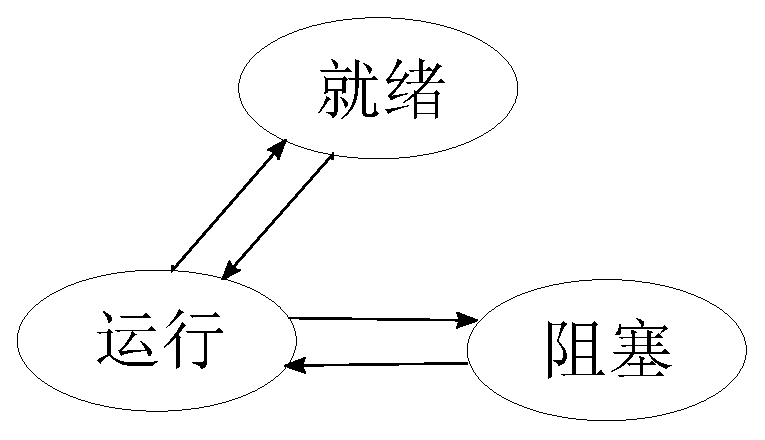
\includegraphics[width=0.5\textwidth]{thread_states}
	\caption{单个线程的状态}
	\label{fig:thread_state}
\end{figure}

通常,在我们接触到的非实时性电脑环境中,中断的行为就是符合一个中断的基本模型。其
行为模式就是简单的抢占当前线程,在执行结束之后恢复上下文继续执行被抢占的线程。

中断处理程序的行为,与多线程程序研究中的线程行为十分相似。我们对中断模型的构建就
参考了多线程程序中的线程模型。如图~\ref{fig:thread_state} 所示,通常,一个线程
会被刻画为以下三个状态。
\begin{itemize}
	\item \emph{就绪}:线程可以运行但是当前并不占有CPU。
	\item \emph{运行}:线程正在运行。
	\item \emph{阻塞}:线程在等待处理器以外的资源,暂时无法运行。
\end{itemize}

由于绝大部分多线程程序研究的场景中,并不关心线程产生和终止。换言之,线程在这类应
用场景里直接存在,且永不终止。中断研究中,一个通常具有一个从产生到终止的完整周期
。而且,一个中断并非只触发一次,因此一个可能重复多次上述周期。这与传统的多线程程
序研究是不同的。所以针对一个,我们类比线程再加以修改可以得到如图~\ref{fig:interrupt_state} 
所示的状态机。每个状态的含义如下。

\begin{figure}[H]
	\centering
	
\includegraphics[width=0.5\textwidth]{interrupt_states}
	\caption{单个中断的状态}
	\label{fig:interrupt_state}
\end{figure}

\begin{itemize}
	\item \emph{无中断}:当前中断没有触发。
	\item \emph{就绪}:中断触发但是有优先级更高的中断在执行。
	\item \emph{运行}:正在运行。
	\item \emph{阻塞}:被优先级更高的中断打断。
\end{itemize}

在多线程的场景中,线程之间的切换往往由线程调度器掌管。线程调度器不是硬件,而是一
段代码,负责实现线程的调度算法。时间片轮转,优先级不同的线程之间的抢占,甚至是线
程优先级的动态变化,都由线程调度器实现。一般而言,线程调度器是系统内核的一重要组
成部分。线程调度器工作的基础就是如图~\ref{fig:thread_table} 所示的线程表结构。
线程表通常是一个二维的表,由系统所支持的线程优先级数构成表的行,每一行内是属于该
优先级的所有线程。通常情况下,系统中会有一个就绪线程表和一个阻塞线程表,当前线程
不在任何一个表中。所有的线程调度算法其实都是对这个表的调整。

\begin{figure}[H]
	\centering
	
\includegraphics[width=0.6\textwidth]{thread_table}
	\caption{线程表}
	\label{fig:thread_table}
\end{figure}

\begin{figure}[H]
	\centering
	
\includegraphics[width=0.25\textwidth]{interrupt_vector_table}
	\caption{中断向量表}
	\label{fig:interrupt_vector_table}
\end{figure}

相比而言,多中断场景比多线程场景简单许多。通常情况下,一个中断优先级对应一个中断
处理程序。所以,中断处理程序的组织形式也是一个表,但是从二维降到了一维。在大部分
文档中,这个表被称为中断向量表(Interrupt Vector Table),如图~\ref{fig:interrupt_vector_table} 
所示。中断向量表中的每个表项被称为一个中断向量(Interrupt Vector),指代一个中
断处理程序。在实现时,一个中断向量通常是一个函数指针,指向某个函数,该函数的内容
就是中断处理。因此,不同于多线程场景中,一个线程优先级可以对应多个线程,如图~
\ref{fig:thread_table}中所示,一个中断优先级对应最多一个中断。中断优先级是由CPU
或外部中断控制器等硬件决定的,实际使用时可能用不到所有的优先级,因此会有大量的中
断向量表项为空。

除了维数降低,中断向量表相比于线程表而言,还有两个不同点。其一,一般而言,中断向
量表在系统初始化完成以后就不再变化。这里的变化指的是已有的中断的优先级变化,即已
有中断在中断向量表中的位置变化。部分操作系统或裸机程序会有在运行时注册或注销中断
的行为,但是从来没有过更改一个现有中断优先级的行为。换言之,在运行时,中断向量表
可以增加或删除表项,但不会更改表项。\footnote{这是一条编程准则。事实上,只要有足
够的权限,更改中断向量表项的操作是被允许的,因而也是可以完成的。只不过大家都不这
么做。}

其二,中断向量表只有一份,包含了所有的中断,不论其当前状态如何。以线程表而言,系
统中可能有两份甚至多份线程表,分别记录不同状态下的线程。除了笼统地将阻塞线程做成
一张线程表,还有一些实现是将请求同一个锁变量的阻塞线程做成一张单独的表。在该实现
下,系统内会同时存在$L+1$张线程表($L$代表系统中锁的数量),另外还有一个当前线程
不在任何线程表内。

到此,一个概念中最基本的中断模型就形成了。中断处理程序状态机如图~\ref{fig:interrupt_state} 
所示,中断间的组织如图~\ref{fig:interrupt_vector_table} 所示。

\subsection{通用的软硬件实现}
\label{subsec:basic_hardware}

为了更加忠实地构建模型,我们需要了解中断的实现。因为基本中断模型完全是由硬件实现
的,了解硬件实现的细节能帮我们掌握更多细节,这有助于帮助我们针对遇到的问题进行合
适的抽象。另一方面,虽然中断的实现完全依赖硬件,但是各个硬件平台在实现上述基本中
断机制的方法大同小异,因此本节将介绍一种通用的实现。

中断的硬件实现最主要两个部分是的中断控制器和中断向量表。

中断控制器在\ref{sec:intr}节有简要的介绍。无论是CPU内部还是外部的控制器,其控
制逻辑都是类似的。通常,CPU会有一个或多个指示当前各种状态的STATUS寄存器。STATUS
寄存器中有一位表示是否有中断需要处理,我们称其为中断标志位。CPU在每一个指令周期
之后会检查中断标志位是否置位,如果置位,CPU会和中断控制器通信获取中断号,然后保
存当前上下文,即将上下文压栈,如图~\ref{fig:stack} 所示\footnote{上下文的具体
内容视不同硬件平台决定,图中只作示意。}。程序计数器(PC)加载中断向量表中对应表项
所指向的中断处理程序地址,开始执行中断程序。进入中断处理时,CPU还会修改STATUS寄
存器中的其他的位以表示它现在正在处理中断。相应的,中断控制器上会有寄存器修改指示
当前所有的中断的状态。在接受新的中断触发信号之后,中断控制器内部的判定逻辑会决定
该中断是否可以立即抢占CPU,进而决定是否需要将CPU的STATUS寄存器中的中断标志位置
位。

\begin{figure}[H]
	\centering
	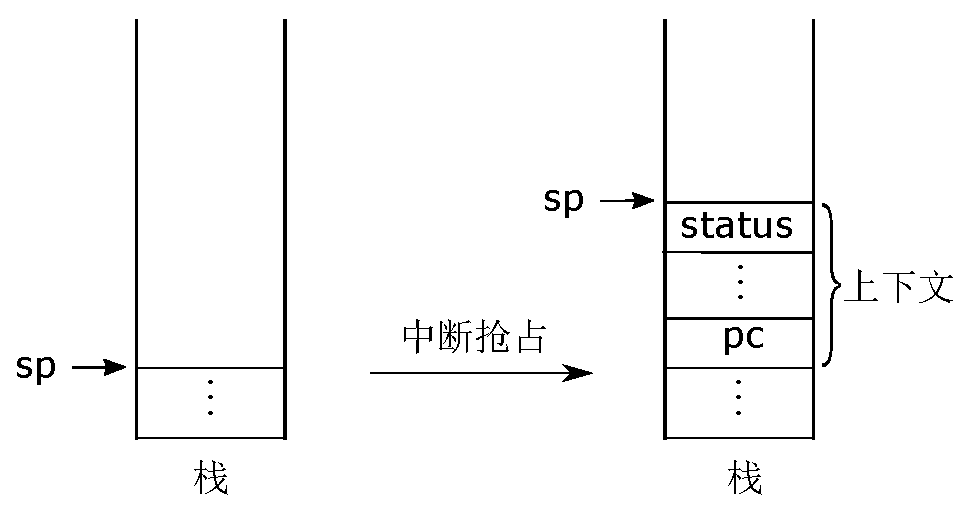
\includegraphics[width=0.9\textwidth]{stack}
	\caption{中断发生前后的栈变化}
	\label{fig:stack}
\end{figure}

中断向量表简单许多。通常,中断向量表是在内存中一块独立的区域。在许多平台上,这块
区域从0x0000\footnote{这里用16位数只是举例,表示在内存首地址。如果在32位或64位
平台,地址应该写成0x0000 0000和0x0000 0000 0000 0000}开始。因为CPU会根据一个
中断向量号来查找对应表项,因此中断向量表的基地址完全由CPU的硬件实现规定。部分CPU
允许在系统初始化的时候重新选择中断向量表的基地址,其原理就在于在这些CPU寻址中断
处理程序时,中断向量表基地址是从一个内部寄存器中取出。通过特定的汇编语句可以修改
该寄存器的值,这就完成了中断向量表基地址的修改。在硬件上电启动之前,中断向量表里
的表项并未被赋值。上电之后,在初始化时,由软件给中断向量表各个用到的表项填上对应
的值,通常是各中断处理函数的函数指针。

\subsection{Uppaal中的基本中断模型}
\label{subsec:basic_uppaal}

在构建中断模型之前,我们首先需要对中断场景做一些必要的简化和抽象,同时辅以合理的
假设,以保证我们最终的问题可解。本文的出发点是多中断相互作用下的中断实时性研究。
中断处理程序的语义我们并不关心,因此中断处理程序的语义可以被忽略。一个中断处理程
序就是一个如图~\ref{fig:interrupt_state} 所示的状态机。而另一方面,我们需要中断
处理的时间。这个时间完全依赖硬件平台,同样的代码换另一套硬件时间会完全不一样,虽
然直观上不同的中断处理的相对时间在不同硬件平台应该保持一致。但事实并非如此。如定
义~\ref{def:intr_time} 中所示,我们需要的中断处理时间$T$。$\tau_1$和$\tau_3$
在同一个硬件平台上针对不同的中断,理论上是一样的。但是$\tau_1$和$\tau_3$在不同
的硬件平台上不一样,这一点很容易理解。$\tau_2$在不同的硬件平台上也不一定会保持同
样的相对关系,也就是说,两段中断处理程序代码在两个不同的硬件平台A和B上的运行时间
的比值$\tau_{2A}/\tau_{2B}$不一定保持一致。这完全依赖于针对两个硬件平台的编译过
程。

\begin{definition}
	中断处理的时间$T$
	\label{def:intr_time}
	\begin{equation}
		T = \tau_1 + \tau_2 + \tau_3
	\end{equation}
	
	$\tau_1$:CPU从检测到中断信号开始到PC跳转到中断处理程序的时间。
	
	$\tau_2$:中断处理程序代码的运行时间。
	
	$\tau_3$:CPU恢复上下文,PC跳转回原执行流的时间。
\end{definition}

因此,在不同的硬件平台,中断处理的时间并没有严格的规律可循,针对一个新的硬件平,
中断处理的时间只能通过测试获得。我们在构建中断模型时,需要将中断处理时间纳入模型
中。又因为中断处理时间只能通过测试获得,我们需要将其参数化以保证我们的模型适用性
更好。

除了中断处理时间$T$,我们还应该关心另一个时间 \pozhehao 中断响应耗时$T^\prime$。
注意定义~\ref{def:intr_last} 中开始时刻是中断控制器接收到中断信号的时刻而不是
CPU的检测到中断信号。我们在接下来的建模中会解释这个区别。

\begin{definition}
	中断响应耗时$T^\prime$指从中断控制器收到中断信号时刻开始到当前时刻消耗的时间。
	\label{def:intr_last}
\end{definition}

接下来,一个重要的元素是优先级。如上文所说,中断优先级在运行时保持不变。但是每个
优先级只有一个中断。模型中所有的中断实例都会有一个独特的中断优先级。因此,我们也
可以将中断优先级与中断ID视作同一个变量。事实上,我们也是这么做的。另一方面,由于
对每个中断来说,其优先级都是独一无二的,因此我们无法将优先级作为一个模型中共有的
部分。如同上述的中断处理时间$T$,中断优先级在建模时只能作为一个参数加入Uppaal模
板之中。

以上只描述了~\ref{subsec:basic_hardware} 节中的中断向量表中的内容,模型中还需
要加入中断控制器的内容。得益于Uppaal的模块同步机制,中断控制的机制可以利用中断模
型间的通信来完成。虽然这样的建模与硬件实现有着本质上的不同,中断不再受到一个管理
者实体控制,而是根据一些规则实行了“民主协商自治”。但是,由于“自治”的规则与管理控
制的规则完全相同,因此实现的效果是相同的。

在这里,我们还需要对中断优先级的抢占规则进行进一步的明确。首先我们定义中断优先级
的表示。如定义~\ref{def:pri} 所示,当且仅当$P_{coming} < P_{current}$,发生抢
占。

\begin{definition}
	中断优先级$P$,表示中断优先级的数值,范围为自然数集$\mathbb{N}$,数值越小,
	优先级越高。$P_{current}$表示当前占据CPU的中断的优先级。$P_{coming}$表示当
	前触发的中断的优先级。
	\label{def:pri}
\end{definition}

至此,我们可以在Uppaal中构建基本中断的模型了。按照~\ref{sec:model_combine} 节
中介绍的顺序,现在分别展示模型的各个部分。

\subsubsection{声明}
\label{subsubsec:basic_decl}

\begin{figure}[H]
	\centering
	\begin{lstlisting}
	const int N = 7;
	typedef int[0, N-1] intr_id; 
	chan intr[intr_id];
	urgent broadcast chan prompt, resume;
	bool ISR[intr_id] = {false, false,false,
	false,false,false,false};
	
	typedef int[0,N] Pri;
	Pri get_highest_pri(){
		meta int i;
		for(i = 0; i < N; i++){
			if(ISR[i]){
				return i;
			} 
		}
		return N;
	}
	\end{lstlisting}
	\caption{基本中断模型:声明}
	\label{fig:basic_decl}
\end{figure}

如图~\ref{fig:basic_decl} 所示,第1行定义了中断优先级的总数,代码中的数字只是
一个例子。第2行定义了一个数据类型,它的作用就如它的名字一样,中断ID。同时,它也
是中断的优先级,数字越小,优先级越高。优先级最高的是0号中断。接下来定义信道,第
3行定义了一组通信信道,分别对应每个中断。第4行定义了两个广播信道。普通信道的信号
只能有一个发送者,一个接收者;广播信道则有一个发送者和多个接收者。普通信道的作用
是用于环境触发特定中断,而广播信道就用来实现抢占,或者由被抢占重新占有CPU的效果。
第5行定义了一个布尔变量数组,模拟ISR(Interrupt Service Register)寄存器。这个
寄存器通常是中断控制器的重要组成部分,在不同硬件平台上有不同的名字,甚至可能代表
了多个寄存器。它的作用指示当前有哪几个中断需要处理,包含正在处理的中断。如果某一
个中断尚未处理结束,即该寄存器某一位置位时,同一中断的下一个实例又触发了,在基本
中断模型中,会被忽略。第8-17行定义了一个函数用来获取当前存在的优先级最高的中断的
优先级(或者说ID)。但是,如果ISR数组里的值都是False,即当前没有任意一个中断需要
处理,那么该函数返回N。优先级N不对应任何一个中断,我们可以认为优先级N对应的是普
通代码。

\subsubsection{基本中断模板}
\label{subsubsec:basic_intr}

\begin{figure}[H]
	\centering
	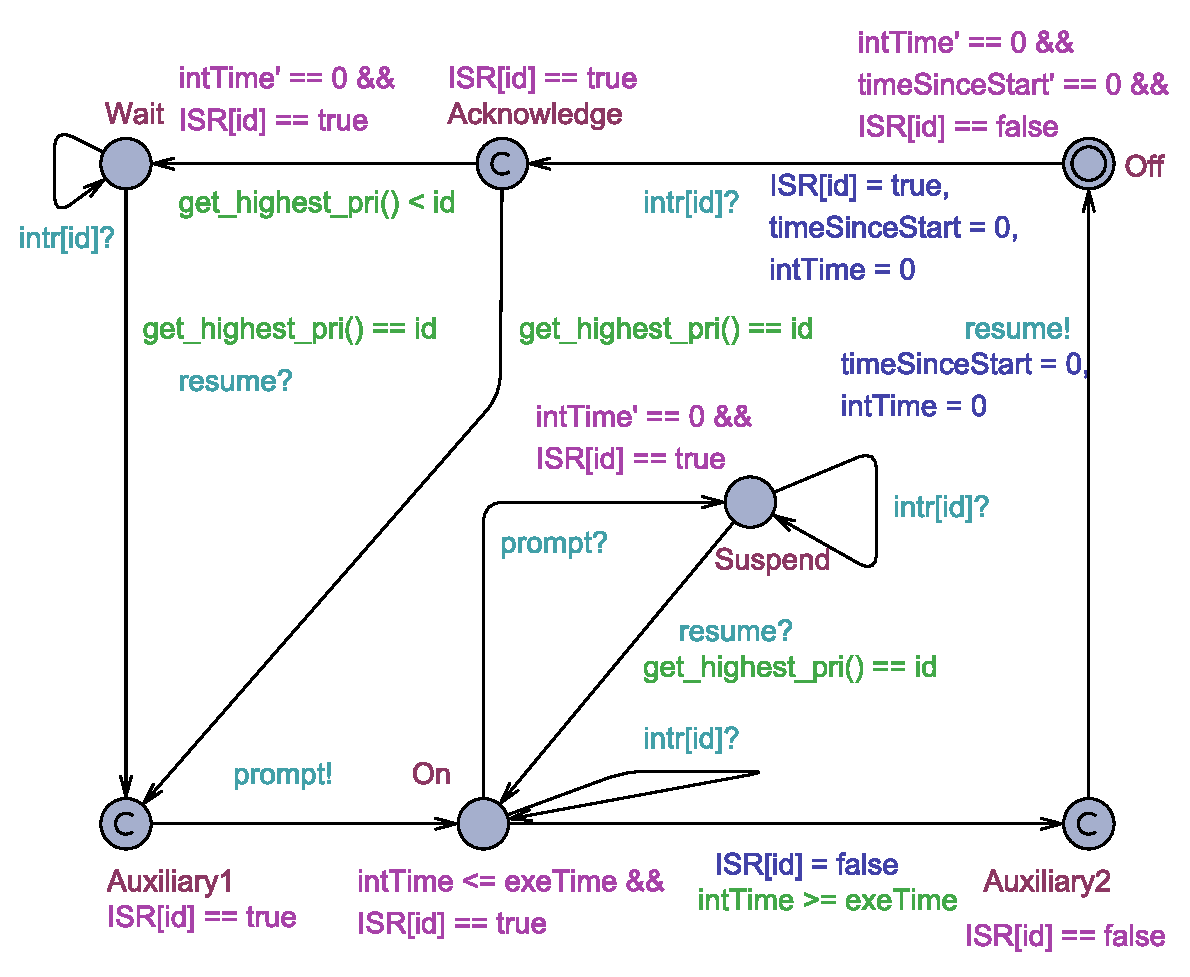
\includegraphics[width=0.9\textwidth]{Interrupt_basic}
	\caption{基本中断:状态机}
	\label{fig:interrupt_basic}
\end{figure}

基本中断的状态机如图~\ref{fig:interrupt_basic} 所示,在这个状态机的状态在Uppaal
中称为位置(Location),以便于整个模型的状态相区分。该模板的内部声明、参数、位置
和变迁的说明分别如表~\ref{tab:basic_intr_decl},表~\ref{tab:basic_intr_para},
表~\ref{tab:basic_intr_loc},表~\ref{tab:basic_intr_mov} 所示。这里,我们定义

\begin{definition}
	\label{def:act_intr_time}
	中断实际处理时间$t$,指从CPU接收到本中断信号开始到当前时刻的时间。
\end{definition}

\begin{table}[htb]
	\centering
	\caption{基本中断模板:内部声明}
	\label{tab:basic_intr_decl}
	\begin{tabularx}{\linewidth}{p{7em}p{5em}X}
		\toprule[1.5pt]
		{\heiti 名称} & {\heiti 类型} & {\heiti 含义}\\
		\midrule[1pt]
		intTime & clock & 中断实际处理时间$t$ \\
		\midrule[0.5pt]
		timeSinceStart & clock & 中断响应耗时$T^\prime$ \\
		\bottomrule[1.5pt]
	\end{tabularx}
\end{table}

\begin{table}[htb]
	\centering
	\caption{基本中断模板:参数}
	\label{tab:basic_intr_para}
	\begin{tabularx}{\linewidth}{p{7em}p{5em}X}
		\toprule[1.5pt]
		{\heiti 名称} & {\heiti 类型} & {\heiti 含义}\\
		\midrule[1pt]
		id & int & 中断号,也是中断优先级 \\
		\midrule[0.5pt]
		exeTime & int & 中断处理时间$T$ \\
		\bottomrule[1.5pt]
	\end{tabularx}
\end{table}

%\begin{table}[!htb]
%	\centering
%	\caption{基本中断模板:位置}
%	\label{tab:basic_intr_loc}
%	\begin{tabularx}{\linewidth}{p{5em}p{5em}p{13em}X}
%		\toprule[1.5pt]
%		{\heiti 名称} & {\heiti 附加属性} & {\heiti 约束} & {\heiti 含义}\\
%		\midrule[1pt]
%		Off & 初始位置 & intTime和timeSinceStart保持静止,ISR对应位为false & 
%		初始位置,当前没有该中断\\
%		\midrule[0.5pt]
%		Acknowledge & 关键位置 & ISR对应位为true & 中断控制器接收到中断信号\\
%		\midrule[0.5pt]
%		Wait & & intTime保持静止,ISR对应位为true & 当前有优先级更高的中断在运
%		行,本中断等待。\\
%		\midrule[0.5pt]
%		Auxiliary1 & 关键位置 & ISR对应位为true & 为表达Wait和Acknowledge到On
%		的语义设置的辅助位置\\
%		\midrule[0.5pt]
%		On & & intTime不超过exeTime,ISR对应位为true & 中断正在被处理 \\
%		\midrule[0.5pt]
%		Suspend & & intTime静止,ISR对应位为true & 中断被更高优先级抢占CPU \\ 
%		\midrule[0.5pt]
%		Auxiliary2 & 关键位置 & ISR对应位为false & 为表达On到Off的完整语义设置
%		的辅助位置\\
%		\bottomrule[1.5pt]
%	\end{tabularx}
%\end{table}

\begin{longtabu} to \linewidth {p{5em}p{5em}p{13em}X}
	\caption{基本中断模板:位置}
	\label{tab:basic_intr_loc}\\
	\toprule[1.5pt]
	{\heiti 名称} & {\heiti 附加属性} & {\heiti 约束} & {\heiti 含义}\\
	\midrule[1pt]
	\endfirsthead
	\multicolumn{4}{c}{续表~\thetable\hskip1em 基本中断模板:位置}\\
	\toprule[1.5pt]
	{\heiti 名称} & {\heiti 附加属性} & {\heiti 约束} & {\heiti 含义}\\
	\midrule[1pt]
	\endhead
	\hline
	\multicolumn{4}{r}{续下页}
	\endfoot
	\endlastfoot
	Off & 初始位置 & intTime和timeSinceStart保持静止,ISR对应位为false & 
	初始位置,当前没有该中断\\
	\midrule[0.5pt]
	Acknowledge & 关键位置 & ISR对应位为true & 中断控制器接收到中断信号\\
	\midrule[0.5pt]
	Wait & & intTime保持静止,ISR对应位为true & 当前有优先级更高的中断在运
	行,本中断等待。\\
	\midrule[0.5pt]
	Auxiliary1 & 关键位置 & ISR对应位为true & 为表达Wait和Acknowledge到On
	的语义设置的辅助位置\\
	\midrule[0.5pt]
	On & & intTime不超过exeTime,ISR对应位为true & 中断正在被处理 \\
	\midrule[0.5pt]
	Suspend & & intTime静止,ISR对应位为true & 中断被更高优先级抢占CPU \\ 
	\midrule[0.5pt]
	Auxiliary2 & 关键位置 & ISR对应位为false & 为表达On到Off的完整语义设置
	的辅助位置\\
	\bottomrule[1.5pt]
\end{longtabu}

\begin{longtabu} to \linewidth {p{5em}p{5em}XXXX}
	\caption{基本中断模板:变迁 }
	\label{tab:basic_intr_mov}\\
	\toprule[1.5pt]
	{\heiti 迁出位置} & {\heiti 迁入位置} & {\heiti 条件} & {\heiti 同步} & 
	{\heiti 更新} & {\heiti 含义}\\
	\midrule[1pt]
	\endfirsthead
	\multicolumn{6}{c}{续表~\thetable\hskip1em 基本中断模板:变迁}\\
	\toprule[1.5pt]
	{\heiti 迁出位置} & {\heiti 迁入位置} & {\heiti 条件} & {\heiti 同步} & 
	{\heiti 更新} & {\heiti 含义}\\
	\midrule[1pt]
	\endhead
	\hline
	\multicolumn{6}{r}{续下页}
	\endfoot
	\endlastfoot
	Off & Acknowledge & & 接收到中断信号 & ISR对应位置位,时钟清零 & 中断控
	制器接收到中断信号\\
	\midrule[0.5pt]
	Acknowledge & Wait & 本中断优先级不是最高 & & & 当前有更高优先级的中断存
	在,本中断等待\\
	\midrule[0.5pt]
	Wait & Auxiliary1 & 本中断优先级最高 & 接收到resume信号 & &  高优先级的
	中断执行完毕,本中断得到CPU\\
	\midrule[0.5pt]
	Wait & Wait & & 接收到中断信号 & & 忽略本中断的其他实例\\
	\midrule[0.5pt]
	Acknowledge & Auxiliary1 & 本中断优先级最高 & & & 本中断优先级最高,准备
	执行\\
	\midrule[0.5pt]
	Auxiliary1 & On & & 发送prompt信号 & & 当前中断获得CPU,打断其他正在被处
	理的中断\\
	\midrule[0.5pt]
	On & Suspend & & 接收到prompt信号 & & 当前中断被更高优先级的中断打断\\
	\midrule[0.5pt]
	On & On & & 接收到中断信号 & & 忽略本中断的其他实例\\
	\midrule[0.5pt]
	Suspend & On & 本中断优先级最高 & 接收到resume信号 & & 高优先级的中断执
	行完毕,本中断得到CPU\\
	\midrule[0.5pt]
	Supend & Suspend & & 接收到中断信号 & & 忽略本中断的其他实例\\
	\midrule[0.5pt]
	On & Auxiliary2 & 中断实际处理时间$t$达到中断处理时间$T$ & & ISR对应位
	复位 & 中断执行结束\\
	\midrule[0.5pt]
	Auxiliary2 & Off & & 发送resume信号 & 时钟清零 & 通知其他中断获取CPU\\
	\bottomrule[1.5pt]
\end{longtabu}

注意,表~\ref{tab:basic_intr_mov} 中并没有选择一列,因为在该模板中,所有的位置
变迁都没有规定选择属性。

\subsubsection{环境模板}
\label{subsubsec:basic_env}

环境实例的作用是提供一个中断触发源。在本模型中,由于没有其他的规定,中断的触发方
式为随机触发。如图~\ref{fig:evn_basic} 所示,环境模板没有内部声明,只有一个位
置,无实际意义,其存在是为了在变迁中随机向intr[0]至intr[N-1]的信道中发送一个信
号。

\begin{figure}[H]
	\centering
	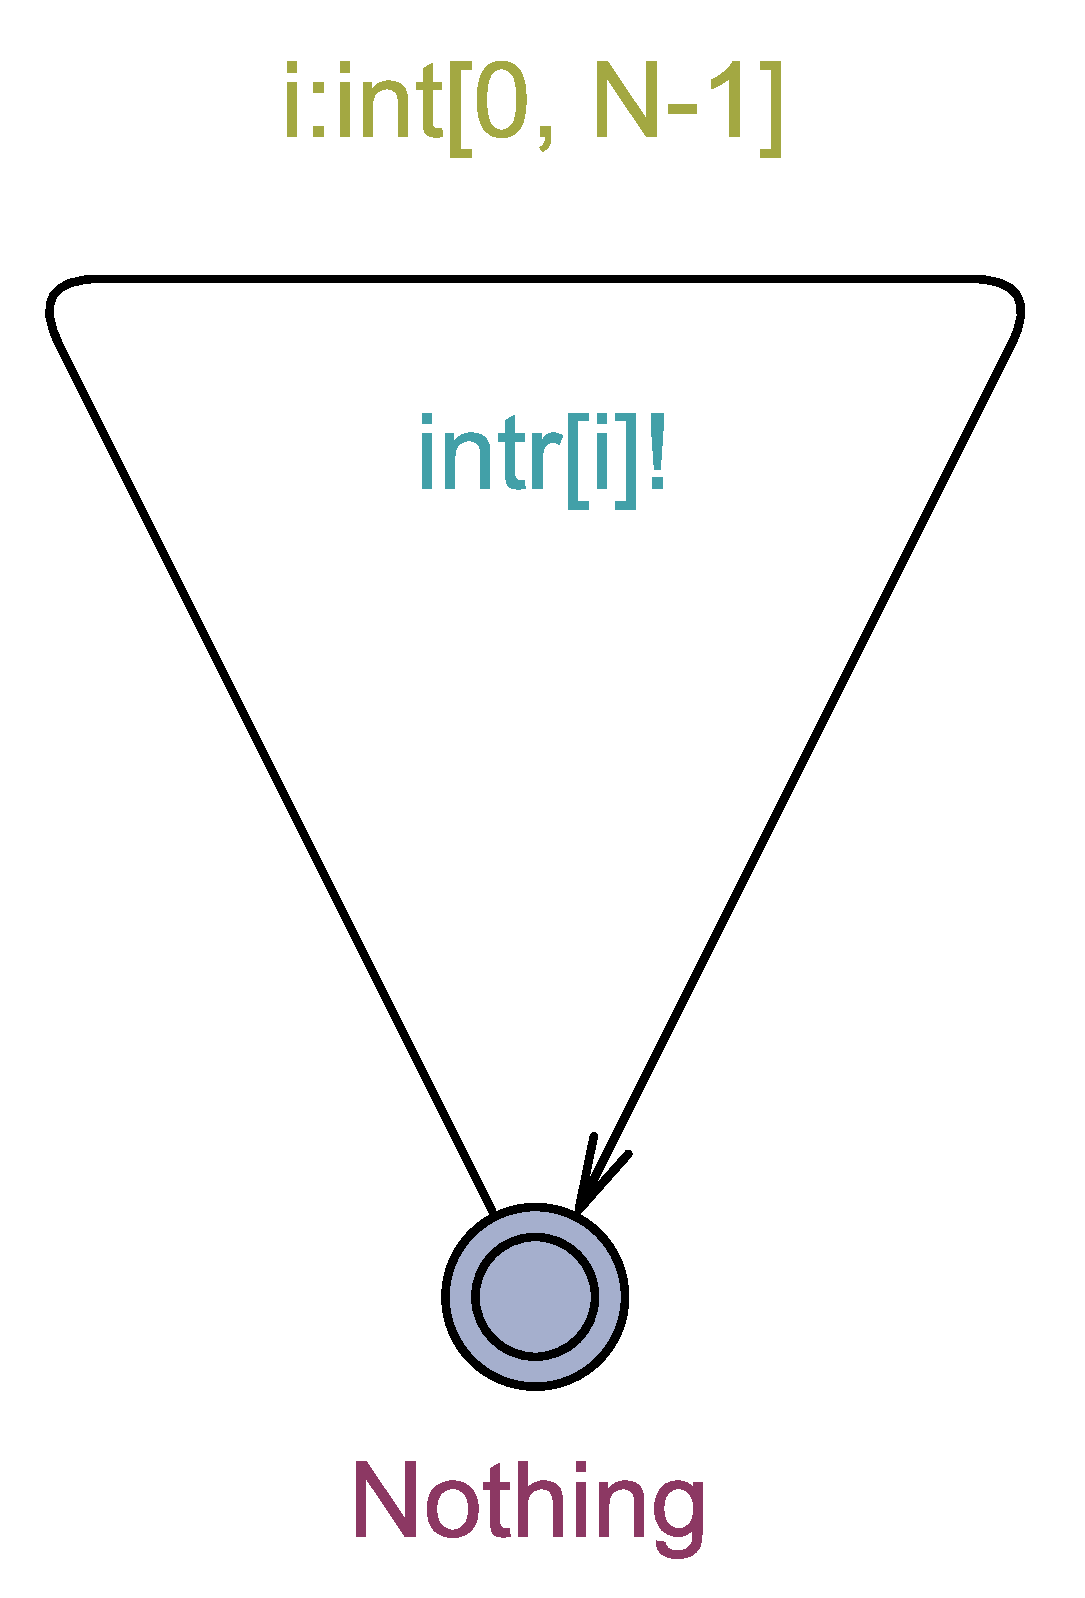
\includegraphics[width=0.2\textwidth]{env_basic}
	\caption{基本中断:环境}
	\label{fig:evn_basic}
\end{figure}

\subsubsection{模型声明}
\label{subsubsec:basic_model_decl}

\begin{figure}[H]
	\centering
	\begin{lstlisting}
	intr0 = Interrupt_basic(0, 1000);
	intr1 = Interrupt_basic(1, 500);
	intr2 = Interrupt_basic(2, 500);
	intr3 = Interrupt_basic(3, 600);
	intr4 = Interrupt_basic(4, 700);
	intr5 = Interrupt_basic(5, 800);
	intr6 = Interrupt_basic(6, 900);
	
	env_basic = env_basic();
	
	system intr0, intr1, intr2, intr3, intr4, 
			intr5, intr6, env_basic;
	\end{lstlisting}
	\caption{基本中断模型:模型声明}
	\label{fig:basic_model_decl}
\end{figure}

在模型声明中我们将声明所有的实例和模型组成。如图~\ref{fig:basic_model_decl} 所示,
1-7行声明了7个中断实例,注意他们的两个参数,分别对应中断ID和中断处理时间$T$。第9
行生命了中断源。第11行声明了整个模型。至此,我们可以进行仿真模拟,撰写性质交给验
证器去验证。

\section{带重入的中断模型}
\label{sec:reentrant}

在~\ref{subsubsec:basic_decl} 小节中,我们提到当一个中断尚未处理完成,它的下一
个实例到来,在基本中断模型中,下一个实例将会被忽略。如果某中断的下一个实例能够抢
占前一个实例,我们就称该中断支持重入(re-entrance)。许多中断平台现在已经支持中
断重入,也有许多软件产品使用了中断重入这个特性。所以如果不能支持重入,那么对中断
模型的限制就有点过分了。

然后,支持重入的中断是不限定重入的次数的。这由其实现机制导致,我们将在
~\ref{subsec:reentrant_hardware} 小节详细讲解。但是,按照我们对基本中断模型的
建模思想,无限制的重入意味着有无限多个模板实例,这些实例将在模型运行中被动态地创
建,这在Uppaal中是不被允许的。同时,这样做还会导致状态本身无限增加,状态空间则是
无穷大,这在模型检测理论中也是不被允许的。因此,我们在建模带重入的中断时,只能退
而求其次,规定重入次数的上限,那么状态大小就是确定的,就可以应用模型检测的理论和
Uppaal来建模。

\subsection{重入的软硬件实现}
\label{subsec:reentrant_hardware}

重入中断的实现非常简单。它与~\ref{subsec:basic_hardware} 小节中描述的基本中断
的通用实现基本相同。差别仅在于中断控制器的优先级判断规则。按照定义~\ref{def:pri} ,
基本中断的抢占条件是$P_{coming} < P_{current}$,而重入中断的抢占条件则是
$P_{coming} \leq P_{current}$。在此条件下,中断可以被自身打断,即发生了自抢占,
在中断处理程序执行结束之前,程序计数器PC又被设置到了同一段中断处理程序的入口,这
也是重入这个术语的来源。

如果我们从栈(Stack)的角度来看中断重入,会发现重入与非重入的抢占在栈的行为上是完
全一致。在~\ref{subsec:basic_hardware} 小节中我们描述了中断抢占发生时上下文会被
压栈。重入时栈上的行为与图~\ref{fig:stack} 完全一致。由此可见,重入的次数没有任何
理论上的限制。在真实的硬件平台上,因为栈溢出是不允许的,重入的次数受栈大小的限制,
然而这也是中断嵌套的层数限制,本质上与中断是否重入没有关系。

\subsection{Uppaal中的重入中断模型}
\label{subsec:reentrant_uppaal}

尽管重入中断和基本中断的实现几乎完全相同,但是由于重入这个行为与基本中断的行为大
相径庭,我们不能简单套用简单中断的模板。通过上文的分析我们知道,对重入中断建模需
要假设重入次数的上限,同时,该上限在实际的硬件平台上是存在的。因此只要设置的合理,
带次数上限的重入中断模型能够反映真实的带重入中断的系统。于是,我们引入假设
~\ref{assume:limit} 。

\begin{assumption}
	带重入的中断系统存在重入次数上限$M$,表示系统中同时存在被处理的同中断实例个数。
	\label{assume:limit}
\end{assumption}

\subsubsection{声明}
\label{subsubsec:reentrant_decl}

首先还是声明部分。我们在基本中断模型的基础上根据假设~\ref{assume:limit} 做了一些
修改。如图~\ref{fig:reentrant_decl} 所示,第2行定义了重入次数上限$M$的取值。第5行
定义了一个相关的数据类型clock\_id。其他定义与~\ref{subsubsec:basic_decl} 小节相
同,本小节不再赘述。

\begin{figure}[H]
	\centering
	\begin{lstlisting}
	const int N = 7;
	const int M = 3;
	
	typedef int[0, N-1] intr_id; 
	typedef int[0, M-1] clock_id;
	chan intr[intr_id];
	urgent broadcast chan prompt, resume;
	
	bool ISR[intr_id] = {false, false,false,false,false,false,false};
	
	typedef int[0,N] Pri;
	Pri get_highest_pri(){
		meta int i;
		for(i = 0; i < N; i++){
			if(ISR[i]){
				return i;
			} 
		}
		return N;
	}
	\end{lstlisting}
	\caption{重入中断模型:声明}
	\label{fig:reentrant_decl}
\end{figure}

\subsubsection{重入中断模板}
\label{subsubsec:reentrant_intr}
重入中断模板在构建的总体思路上还是遵照了图~\ref{fig:thread_state} ,但是在细节上,
尤其是运行状态,重入中断模板做了很大的扩充以支持重入这一特性。重入中断的状态机如图
~\ref{fig:Interrupt_reentrant} 所示,表示运行的位置由一个变成了三个。这是因为在
这个模型中重入次数上限$M$的取值为3。如果$M==4$,那么就需要第四个运行位置。即,$M$
决定了代表运行的位置数。这么做的原因是Uppaal限制了迁移的Guard中,有关时钟的语义范
围,且当重入次数发生改变时,无法用纯静态的循环表达式表达出限制要求。这样添加位置数
的做法使得状态机不够简洁,不过这是我目前能够想到得最合理的建模方式。

\begin{table}[htb]
	\centering
	\caption{重入中断模板:内部声明}
	\label{tab:reentrant_intr_decl}
	\begin{tabularx}{\linewidth}{p{7em}p{5em}X}
		\toprule[1.5pt]
		{\heiti 名称} & {\heiti 类型} & {\heiti 含义}\\
		\midrule[1pt]
		current & clock\_id & 当前占据CPU的中断实例ID,初始为0 \\
		\midrule[0.5pt]
		intTime[M] & clock数组 & 对应每个重入中断实例的中断实际处理时间$t$ \\
		\midrule[0.5pt]
		timeSinceStart[M] & clock数组 & 对应每个重入中断实例的中断响应耗时$T^\prime$ \\
		\midrule[0.5pt]
		initClock & 无返回值的函数 & 将所有时钟清零 \\
		\bottomrule[1.5pt]
	\end{tabularx}
\end{table}

%\begin{longtabu} to \linewidth {p{7em}p{5em}X}
%	\caption{重入中断模板:内部声明}
%	\label{tab:reentrant_intr_decl}\\
%	\toprule[1.5pt]
%	{\heiti 名称} & {\heiti 类型} & {\heiti 含义}\\
%	\midrule[1pt]
%	\endfirsthead
%	\multicolumn{3}{c}{续表~\thetable\hskip1em 重入中断模板:内部声明}\\
%	\toprule[1.5pt]
%	{\heiti 名称} & {\heiti 类型} & {\heiti 含义}\\
%	\midrule[1pt]
%	\endhead
%	\hline
%	\multicolumn{3}{r}{续下页}
%	\endfoot
%	\endlastfoot
%	intTime[$M$] & clock数组 & 对应每个重入中断实例的中断实际处理时间$t$ \\
%	\midrule[0.5pt]
%	timeSinceStart[$M$] & clock数组 & 对应每个重入中断实例的中断响应耗时$T^\prime$ \\
%	\midrule[0.5pt]
%	initClock & 无返回值的函数 & 将所有时钟清零 \\
%	\bottomrule[1.5pt]
%\end{longtabu}

\begin{figure}[H]
	\centering
	\begin{lstlisting}
	void initClock(){
		meta int i;
		for(i = 0; i < M; i++){
			intTime[i] = 0;
			timeSinceStart[i] = 0;
		}
	}
	\end{lstlisting}
	\caption{initClock函数定义}
	\label{fig:initClock}
\end{figure}

\begin{table}[htb]
	\centering
	\caption{重入中断模板:参数}
	\label{tab:reentrant_intr_para}
	\begin{tabularx}{\linewidth}{p{7em}p{5em}X}
		\toprule[1.5pt]
		{\heiti 名称} & {\heiti 类型} & {\heiti 含义}\\
		\midrule[1pt]
		id & int & 中断号,也是中断优先级 \\
		\midrule[0.5pt]
		exeTime & int & 中断处理时间$T$ \\
		\bottomrule[1.5pt]
	\end{tabularx}
\end{table}

除了位置的数量以外,模板内部的声明和状态机上的其他细节也发生了很多变化,为了行文方
便,在此还是依次列出完整的模板声明,参数,位置和变迁,分别见表
~\ref{tab:reentrant_intr_decl} ,表~\ref{tab:reentrant_intr_para},
表~\ref{tab:reentrant_intr_loc},表~\ref{tab:reentrant_intr_mov} 。注意,在
表~\ref{tab:reentrant_intr_decl}提到的函数的定义如图~\ref{fig:initClock} 所示。

\begin{figure}[H]
	\centering
	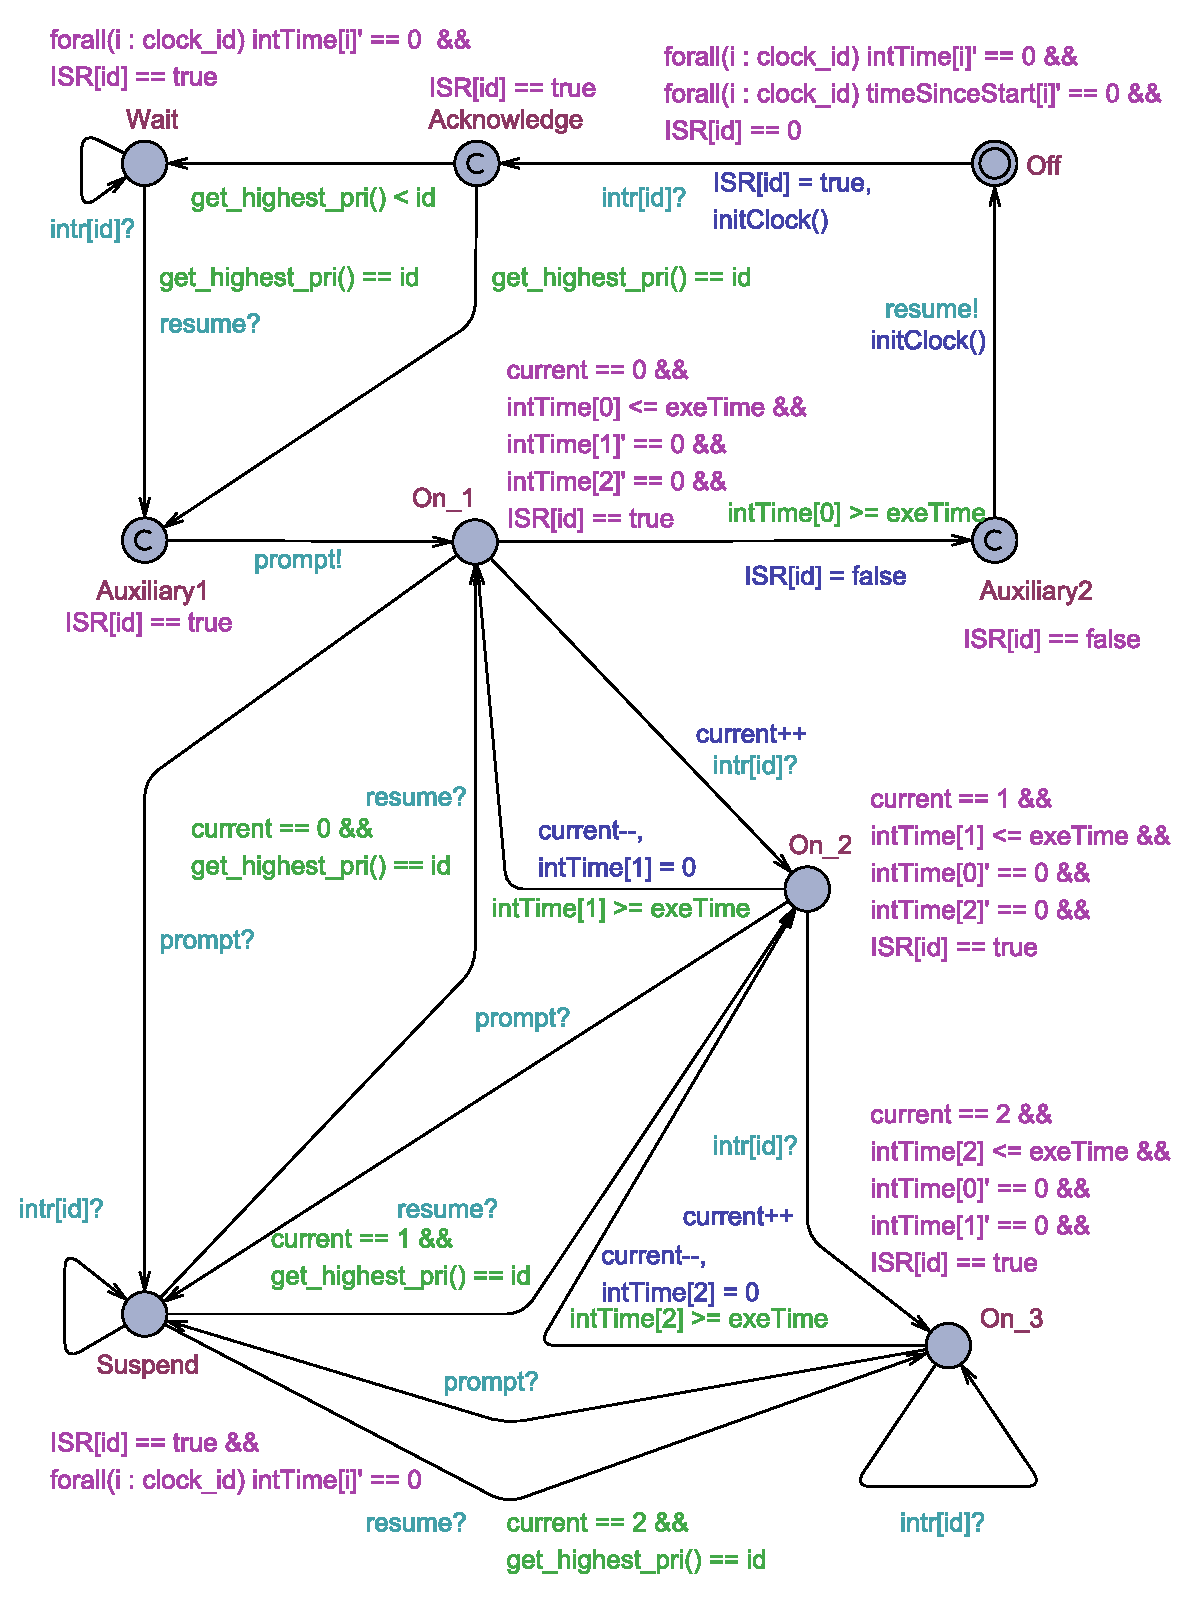
\includegraphics[width=\textwidth]{Interrupt_reentry}
	\caption{重入中断:状态机}
	\label{fig:Interrupt_reentrant}
\end{figure}

\begin{longtabu} to \linewidth {p{5em}p{5em}p{13em}X}
	\caption{重入中断模板:位置}
	\label{tab:reentrant_intr_loc}\\
	\toprule[1.5pt]
	{\heiti 名称} & {\heiti 附加属性} & {\heiti 约束} & {\heiti 含义}\\
	\midrule[1pt]
	\endfirsthead
	\multicolumn{4}{c}{续表~\thetable\hskip1em 重入中断模板:位置}\\
	\toprule[1.5pt]
	{\heiti 名称} & {\heiti 附加属性} & {\heiti 约束} & {\heiti 含义}\\
	\midrule[1pt]
	\endhead
	\hline
	\multicolumn{4}{r}{续下页}
	\endfoot
	\endlastfoot
	Off & 初始位置 & intTime时钟组和timeSinceStart时钟组均保持静止,ISR对应位
	为false & 初始位置,当前没有该中断\\
	\midrule[0.5pt]
	Acknowledge & 关键位置 & ISR对应位为true & 中断控制器接收到中断信号\\
	\midrule[0.5pt]
	Wait & & intTime时钟组保持静止,ISR对应位为true & 当前有优先级更高的中断
	在运行,本中断等待。\\
	\midrule[0.5pt]
	Auxiliary1 & 关键位置 & ISR对应位为true & 为表达Wait和Acknowledge到On\_1
	的语义设置的辅助位置\\
	\midrule[0.5pt]
	On\_1 & & intTime[0]不超过exeTime,ISR对应位为true,其他intTime时钟静止 & 
	中断正在被处理 \\
	\midrule[0.5pt]
	On\_2 & & intTime[1]不超过exeTime,ISR对应位为true,其他intTime时钟静止 & 
	中断被重入一次,正在被处理 \\
	\midrule[0.5pt]
	On\_3 & & intTime[2]不超过exeTime,ISR对应位为true,其他intTime时钟静止 & 
	中断被重入两次,正在被处理 \\
	\midrule[0.5pt]
	Suspend & & intTime静止,ISR对应位为true & 中断被更高优先级抢占CPU \\ 
	\midrule[0.5pt]
	Auxiliary2 & 关键位置 & ISR对应位为false & 为表达On\_1到Off的完整语义设置
	的辅助位置\\
	\bottomrule[1.5pt]
\end{longtabu}

\begin{longtabu} to \linewidth {p{5em}p{5em}XXXX}
	\caption{重入中断模板:变迁 }
	\label{tab:reentrant_intr_mov}\\
	\toprule[1.5pt]
	{\heiti 迁出位置} & {\heiti 迁入位置} & {\heiti 条件} & {\heiti 同步} & 
	{\heiti 更新} & {\heiti 含义}\\
	\midrule[1pt]
	\endfirsthead
	\multicolumn{6}{c}{续表~\thetable\hskip1em 基本中断模板:变迁}\\
	\toprule[1.5pt]
	{\heiti 迁出位置} & {\heiti 迁入位置} & {\heiti 条件} & {\heiti 同步} & 
	{\heiti 更新} & {\heiti 含义}\\
	\midrule[1pt]
	\endhead
	\hline
	\multicolumn{6}{r}{续下页}
	\endfoot
	\endlastfoot
	Off & Acknowledge & & 接收到中断信号 & ISR对应位置位,时钟清零 & 中断控
	制器接收到中断信号\\
	\midrule[0.5pt]
	Acknowledge & Wait & 本中断优先级不是最高 & & & 当前有更高优先级的中断存
	在,本中断等待\\
	\midrule[0.5pt]
	Wait & Auxiliary1 & 本中断优先级最高 & 接收到resume信号 & &  高优先级的
	中断执行完毕,本中断得到CPU\\
	\midrule[0.5pt]
	Wait & Wait & & 接收到中断信号 & & 忽略本中断的其他实例\\
	\midrule[0.5pt]
	Acknowledge & Auxiliary1 & 本中断优先级最高 & & & 本中断优先级最高,准备
	执行\\
	\midrule[0.5pt]
	Auxiliary1 & On\_1 & & 发送prompt信号 & & 当前中断获得CPU,打断其他正在被处
	理的中断\\
	\midrule[0.5pt]
	On\_1 & Suspend & & 接收到prompt信号 & & 当前中断被更高优先级的中断打断\\
	\midrule[0.5pt]
	On\_1 & On\_2 & & 接收到中断信号 & current增加1 & 发生第一次重入\\
	\midrule[0.5pt]
	On\_2 & Suspend & & 接收到prompt信号 & & 当前中断被更高优先级的中断打断\\
	\midrule[0.5pt]
	On\_2 & On\_3 & & 接收到中断信号 & current增加1 & 发生第二次重入\\
	\midrule[0.5pt]
	On\_2 & On\_1 & intTime[1]达到exeTime & & current减少1 & 第一次重入处理完毕\\
	\midrule[0.5pt]
	On\_3 & Suspend & & 接收到prompt信号 & & 当前中断被更高优先级的中断打断\\
	\midrule[0.5pt]
	On\_3 & On\_3 & & 接收到中断信号 &  & 忽略以后的本中断实例\\
	\midrule[0.5pt]
	On\_3 & On\_2 & intTime[2]达到exeTime & & current减少1 & 第二次重入处理完毕\\
	\midrule[0.5pt]
	Suspend & On\_1 & 本中断优先级最高 & 接收到resume信号 & & 高优先级的中断执
	行完毕,本中断得到CPU\\
	\midrule[0.5pt]
	Suspend & On\_2 & 本中断优先级最高 & 接收到resume信号 & & 高优先级的中断执
	行完毕,本中断得到CPU\\
	\midrule[0.5pt]
	Suspend & On\_3 & 本中断优先级最高 & 接收到resume信号 & & 高优先级的中断执
	行完毕,本中断得到CPU\\
	\midrule[0.5pt]
	Supend & Suspend & & 接收到中断信号 & & 忽略本中断的其他实例\\
	\midrule[0.5pt]
	On\_1 & Auxiliary2 & intTime[0]达到exeTime & & ISR对应位复位 & 中断执行结束\\
	\midrule[0.5pt]
	Auxiliary2 & Off & & 发送resume信号 & 时钟清零 & 通知其他中断获取CPU\\
	\bottomrule[1.5pt]
\end{longtabu}

在这个模型中,中断重入只有在本中断是当前优先级最高的中断时才会发生。如果本中断的优先级
较低,那么本中断会处于Wait或者Suspend的位置,中断重入就无法发生。因为一旦发生重入,如
果在运行的位置,就会造成优先级反转;如果在Wait或者Suspend位置,就会发生某个中断的多个
实例在等待。这两者都不符合中断系统的设置和硬件的实现。

\subsubsection{环境模板}
\label{subsubsec:reentrant_env}
这个模型中的环境模板与~\ref{subsubsec:basic_env} 小节中描述的完全一致,在此不赘述。

\subsubsection{模型声明}
\label{subsubsec:reentrant_model_decl}
模型声明与~\ref{subsubsec:basic_model_decl} 小节中描述的基本相似,见
图~\ref{fig:reentrant_model_decl} 。

\begin{figure}[H]
	\centering
	\begin{lstlisting}
	intr0 = Interrupt_reentry(0, 1000);
	intr1 = Interrupt_reentry(1, 500);
	intr2 = Interrupt_reentry(2, 500);
	intr3 = Interrupt_reentry(3, 600);
	intr4 = Interrupt_reentry(4, 700);
	intr5 = Interrupt_reentry(5, 800);
	intr6 = Interrupt_reentry(6, 900);
	
	env = env_reentry();
	
	system intr0, intr1, intr2, intr3, intr4, 
			intr5, intr6, env;   
	\end{lstlisting}
	\caption{重入中断模型:模型声明}
	\label{fig:reentrant_model_decl}
\end{figure}

\section{分段中断模型}
\label{sec:segment}

在~\ref{subsec:intr_OS} 小节中,我们已经提到了分段中断。如图~\ref{fig:ecos_intr_exec} 所
示的中断正是分段中断。此类中断多见于嵌入式应用场景。分段中断的出现从嵌入式开发
的角度来讲,极大地方便了应用的开发,可以在不牺牲实时性的同时让中断完成更繁重的任务。
这一点在开发中断驱动程序(Interrupt-driven Program)的时候极为重要。中断驱动程序
的主要功能都是在中断中完成。如果功能比较复杂或者牵涉到与其他硬件的交互,不可避免地,
中断处理时间会比较长。在没有分段处理的情况下,低优先级的中断的响应时间将大为增加,
实时性无法保证。

另一方面,分段中断对程序分析和验证带来了很大的困难。中断原本的不确定性就足以使任何
针对中断程序的验证,尤其是形式化验证的工作量和难度接近或者超出现有工具和人力的极限。
如果中断程序可以分段,且两段程序在执行上还有一些不同(例如优先级不同),那么分析的
难度将呈指数级增长。幸运的是,如果只着眼于实时性分析,在中断分段以后两段间只有优先
级不同的情况下,我们还是可以用近似的方法去建模和验证的。

\subsection{软件的二次实现}
\label{subsec:segment_software}

在~\ref{subsec:intr_OS} 小节中,我们提到了分段中断是操作系统系统的二次实现。这也
是为了实现实时性需求嵌入式开发程序员在硬件平台不支持分段中断的情况下做出的机智创作。
市面上多家实时操作系统提供了分段中断的机制。在此我会着重介绍eCos操作系统的分段中断
机制。详细了解过操作系统的实现之后,经过适当的抽象,我们可以在Uppaal内对分段中断构
建自动机模型。

eCos是一个跨平台的操作系统,支持各类CPU和板载中断控制器。不同平台对应的汇编代码并
不一样,在此我仅以ARM提供的Cortex M系列CPU为硬件平台讲解eCos的分段中断机制。

\subsubsection{Cortex M系列CPU的中断机制}
\label{subsubsec:cortex_m}

Cortex M系列CPU采用ARMv7-M体系结构,该体系结构针对移动平台设计,在能耗上相当好的
控制。在中断\footnote{在ARMv7-M Architecture Reference Manual中,ARM称本文所说
的中断为异常(Exception),其中,0-15号异常为预定义好的,其处理程序也已固化在硬件
上,16号以后的异常被称为中断(Interrupt)。这只是术语的不同,为了防止混淆,在本文
中统称中断(Interrupt)。}控制机制上,ARMv7-M体系结构与~\ref{subsec:basic_hardware} 小
节所述类似,也采用在栈上保存上下文,进入中断处理之后结束再恢复上下文。但是细节上有
很多ARM平台特有的细节,我会尽量简单的描述这些细节,以便读者能够更好地理
解~\ref{subsubsec:ecos_intr} 小节中的内容。

ARMv7-M体系结构包含13个通用寄存器,R0-R12,以及3个额外的特殊寄存器。

\begin{description}
	\item[SP] 栈指针,用来指示当前活跃的栈的顶部内存位置。SP有时也被称为
	R13。
	\item[LR] 链接寄存器,用来保存返回链接。返回链接是指进行了一次带返回
	的跳转指令的返回地址,通常是跳转指令的下一条指令。该寄存器的复位值为0xFFFFFFFF,
	使用该值进行跳转返回会触发一个错误。LR寄存器在进入中断时也会更新,我们会在下
	文描述。LR有时也被称为R14。
	\item[PC] 程序计数器。PC有时也被称为R15。
\end{description}

在ARMv7-M体系结构中,内存中同时存在两个栈空间\pozhehao 线程栈\footnote{准确的译
名应为进程栈(Process Stack),为行文方便,在此不区分进程和线程。}和主栈,线程栈
属于当前线程,主栈则是所有程序共用。尽管每个线程都有一个自己的线程栈,但是SP所指
向的线程栈是当前线程栈,因此不会发生混淆。CPU内有两个特殊寄存器。

\begin{description}
	\item[PSP] 线程栈指针,永远指向当前线程栈的栈顶。
	\item[MSP] 主栈指针,永远指向主栈栈顶。
\end{description}

SP的读取值可以是PSP的值也可以是MSP的值,即PS可以指向当前线程栈栈顶也可以指向主栈
栈顶,这取决于专用CONTROL寄存器的SPSEL位(即第1位)的当前值。如果为CONTROL.SPSEL
的值为0,SP指向主栈栈顶;如果CONTROL.SPSEL的值为1,SP指向线程栈栈顶。CPU有线程模
式(Thread Mode)和处理模式(Handler Mode),在线程模式下,CONTROL.SPSEL的取值
可以是0或1;在处理模式下,CONTROL.SPSEL的读取值永远为0。换句话说,在线程模式下,
SP可以指向线程栈或主栈,但是在处理模式下,SP永远指向主栈。CPU在接收中断时会进入处
理模式。

在CPU接收到中断信号的,它会将8个32为寄存器压栈,包括xPSR寄存器,返回地址,LR,R12,
R3,R2,R1和R0。这与CPU在执行函数调用时遵守的ARM Architecture Procedure Calling
Standard(AAPCS)保持一致。在进入中断时,LR会被写入一个特殊的值\textbf{EXC\_RETURN}。
因为返回地址和LR原本的值都已经被压栈保存起来,因此LR在中断处理时空闲出来。中断处理
时,返回的标志就是向PC寄存器中写入EXC\_RETURN。一般情况下,写入的EXC\_RETURN就是
LR中保存的值,也可以是从其他途径得到的值。EXC\_RETURN的取值固定且分别具有不同的含
义,如表~\ref{tab:exe_return_noFP} 和表~\ref{tab:exe_return_FP} 所示。在
表~\ref{tab:exe_return_FP} 中的帧类型是指浮点数扩展模式下触发中断时压入栈的寄存器
构成的帧类型。有无浮点数支持,上述8个寄存器都会被压栈,且接下来的分析也只需要用到
它们,因此浮点数的模式在此不做单独讨论。\cite{ARM} 

\begin{table}[htb]
	\centering
	\caption{EXC\_RETURN定义的中断返回行为,无浮点扩展}
	\label{tab:exe_return_noFP}
	\begin{tabularx}{\linewidth}{XXX}
		\toprule[1.5pt]
		{\heiti EXC\_RETURN} & {\heiti 返回到模式} & {\heiti 返回到栈}\\
		\midrule[1pt]
		0xFFFFFFF1 & 处理模式 & 主栈 \\
		\midrule[0.5pt]
		0xFFFFFFF9 & 线程模式 & 主栈 \\
		\midrule[0.5pt]
		0xFFFFFFFD & 线程模式 & 线程栈 \\
		\bottomrule[1.5pt]
	\end{tabularx}
\end{table}

\begin{table}[htb]
	\centering
	\caption{EXC\_RETURN定义的中断返回行为,有浮点扩展}
	\label{tab:exe_return_FP}
	\begin{tabularx}{\linewidth}{XXXX}
		\toprule[1.5pt]
		{\heiti EXC\_RETURN} & {\heiti 返回到模式} & {\heiti 返回到栈} &
		{\heiti 帧类型}\\
		\midrule[1pt]
		0xFFFFFFE1 & 处理模式 & 主栈 & 扩展\\
		\midrule[0.5pt]
		0xFFFFFFE9 & 线程模式 & 主栈 & 扩展\\
		\midrule[0.5pt]
		0xFFFFFFED & 线程模式 & 线程栈 & 扩展\\
		\midrule[0.5pt]
		0xFFFFFFF1 & 处理模式 & 主栈 & 基本\\
		\midrule[0.5pt]
		0xFFFFFFF9 & 线程模式 & 主栈 & 基本\\
		\midrule[0.5pt]
		0xFFFFFFFD & 线程模式 & 线程栈 & 基本\\
		\bottomrule[1.5pt]
	\end{tabularx}
\end{table}

\subsubsection{eCos的分段中断机制} 
\label{subsubsec:ecos_intr}

eCos提供一个分段中断机制。应用程序在注册中断时,可以提供两段程序,分别称为ISR(Immediate
Service Routine)\footnote{注意与本文其他章节里的中断服务寄存器ISR区分,在本小节中涉及的
的所有ISR均指代Immediate Service Routine。}和DSR(Delayed Service Routine)。其中,ISR
在中断触发之后立即被执行的(如果优先级满足条件的话),DSR则会被推迟执行,所有DSR的优先级
低于一切ISR,所有DSR之间的优先级是同等的。\cite{ecos_isr}经过对eCos代码的研读分析,如果
在中断触发时,ISR执行完之后,DSR因故未能执行,那么所有的DSR会在下一次线程切换时全部执行完
毕。这样的好处是显而易见的。应用程序将必须立即处理的不涉及共享资源或者运行时间比较短的部分
放在ISR中处理,把剩下的部分放在DSR里,既充分利用的中断的便利,又不牺牲程序的实时性性能。
\footnote{值得一提的是,应用程序并没有选择使用传统的一段式中断的自由。在逻辑上,程序员只能
把所有中断代码放在ISR中,并提交一个空的DSR来完成传统的一段式中断的行为。此时,操作系统在此
因为DSR的处理反而会消耗相比传统一段式中断更多的CPU周期。}

经过对eCos内核和针对Cortex M系列CPU的HAL(Hardware Abstract Layer, 硬件抽象层)代码的
仔细研读,我们将eCos操作系统的分段中断流程整理成图~\ref{fig:ecos_isr_dsr} 和
图~\ref{fig:ecos_stack} 。下面我们按照图示详细剖析一遍。

\begin{figure}[H]
	\centering
	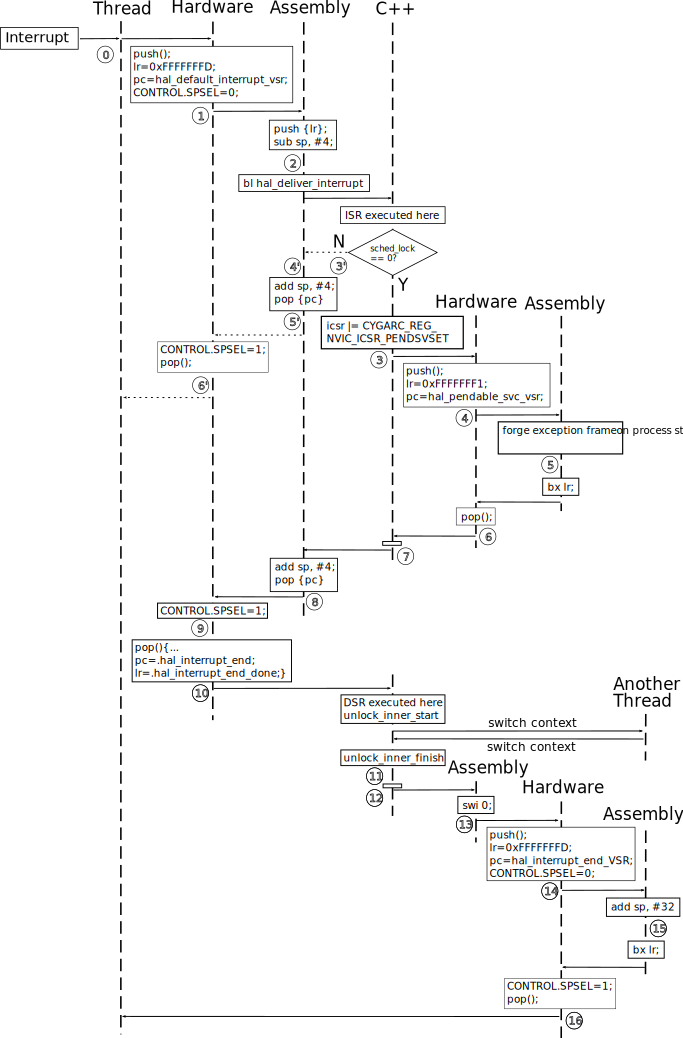
\includegraphics[width=\textwidth]{ecos_isr_dsr}
	\caption{eCos分段中断图解}
	\label{fig:ecos_isr_dsr}
\end{figure}

\begin{figure}[H]
	\centering
	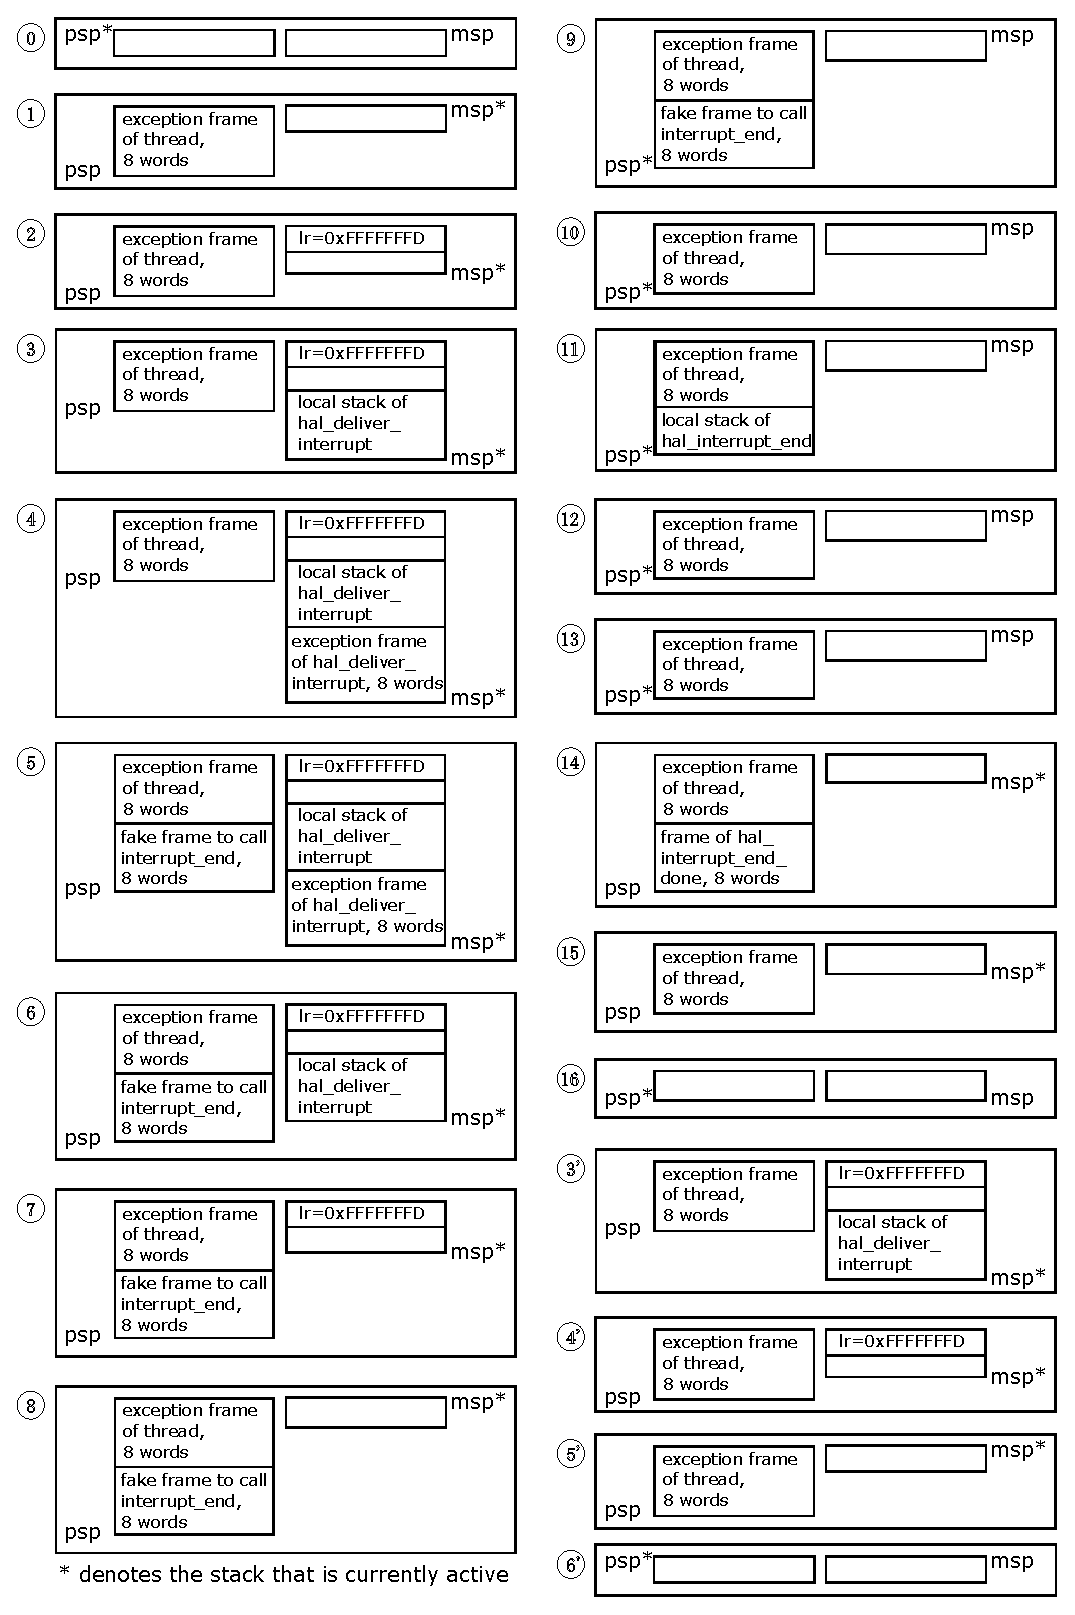
\includegraphics[width=\textwidth]{ecos_stack}
	\caption{eCos分段中断栈情况一览}
	\label{fig:ecos_stack}
\end{figure}

\subsection{Uppaal中的分段中断模型}
\label{subsec:segment_uppaal}

\subsubsection{声明}
\label{subsubsec:segment_decl}

\subsubsection{分段中断模板}
\label{subsubsec:segment_intr}

\subsubsection{环境模板}
\label{subsubsec:segment_env}

\subsubsection{模型声明}
\label{subsubsec:segment_model_decl}

\section{本章小结}
\label{sec:sum_3}
